\clearpage
%%=========================================
\section{MCT Film Grown by LPE on Substrate A}\label{sec:subAc}

A film of \acl{mct} was grown on substrate A by \ac{lpe}. Nomarski optical microscopy images revealed that the surface of the \ac{mct} film was non-planar in the form of wavy structures with a large number of circular features, as seen in Fig.~\ref{fig:subAc_om}. Two different kinds of circular features were observed: large circular defects with diameter of \SIrange{25}{40}{\micro\metre}, as seen in Fig.~\ref{fig:subAc_om_40um}, and donut-shaped defects with a diameter of \SIrange{10}{14}{\micro\metre}, as seen in Fig.~\ref{fig:subAc_om_10um}. %\todo{In addition, some long-distance perturbations in the layer thickness was visible to the naked eye. These are due to solutal convection.}

\begin{figure}[htbp]
    \centering
    \mySubfigure{0.49\textwidth}{LPE453_nomarski_grid_16_20x.jpg}[fig:subAc_om_centre][angle=180]
    \hfill
    \mySubfigure{0.49\textwidth}{LPE453_nomarski_grid_18_20x.jpg}[fig:subAc_om_edge][angle=180]
    \caption[Nomarski phase contrast microscopy images of \ac{mct} film grown by \ac{lpe} on substrate A.]{Nomarski phase contrast microscopy images of \ac{mct} film grown by \ac{lpe} on (111)B-oriented substrate A: \subref{fig:subAc_om_centre} Near the centre; and \subref{fig:subAc_om_edge} near the right edge.}
    \label{fig:subAc_om}
\end{figure}

\begin{figure}[htbp]
    \centering
    \mySubfigure{0.49\textwidth}{LPE453_om_5x_40um.png}[fig:subAc_om_40um][angle=180]
    \hfill
    \mySubfigure{0.49\textwidth}{LPE453_om_10um.png}[fig:subAc_om_10um][angle=180]
    \caption[Bright field optical microscopy images of defects seen on \ac{mct} film grown by \ac{lpe} on substrate A.]{Bright field optical microscopy images of: \subref{fig:subAc_om_40um} \SI{40}{\micro\metre} wide defect; and \subref{fig:subAc_om_10um} donut-shaped defects \SI{10}{\micro\metre} wide seen on \ac{mct} film grown by \ac{lpe} on (111)B-oriented substrate A.}
    \label{fig:subAc_om_40umand10um}
\end{figure}

The wavy structures, called terrace patterns in the litterature, are typical of \ac{lpe} growth and it has been confirmed that these patterns are caused by the misorientation of the substrate surface \citep{benz1980crystals, parker1988terracing}. \citet{li1998crystallinity} showed that the best crystal quality was achieved with growth on \SIrange{1.2}{2}{\degree} off (111)A-oriented substrate. The \ac{lpe} growth performed in this study was not done under these conditions, and consequently, there were a lot of wavy structures.

The large defects were infrequent with respect to the donut-shaped defects. Only four large defects were observed in the lower right quadrant of the sample, which gave a density of \SI{\sim 2}{\centi\metre^{-2}}. The density of donut-shaped defects, on the other hand, was found to be between \SIrange{4e+3}{6e+4}{\centi\metre^{-2}}. The average density was \SI{2e+04}{\centi\metre^{-2}} with a standard deviation of \SI{1e+04}{\centi\metre^{-2}}. A graphical representation of the density at different locations on the film can be seen in Fig.~\ref{fig:LPE453_densityData}. The sample Pearson correlation coefficient between the occurrence of polishing grit on substrate A and the occurrence of donut-shaped defects on the film was determined to be \SI{-0.04}{}, which was a very weak negative correlation.


\begin{figure}[htbp]
    \centering
    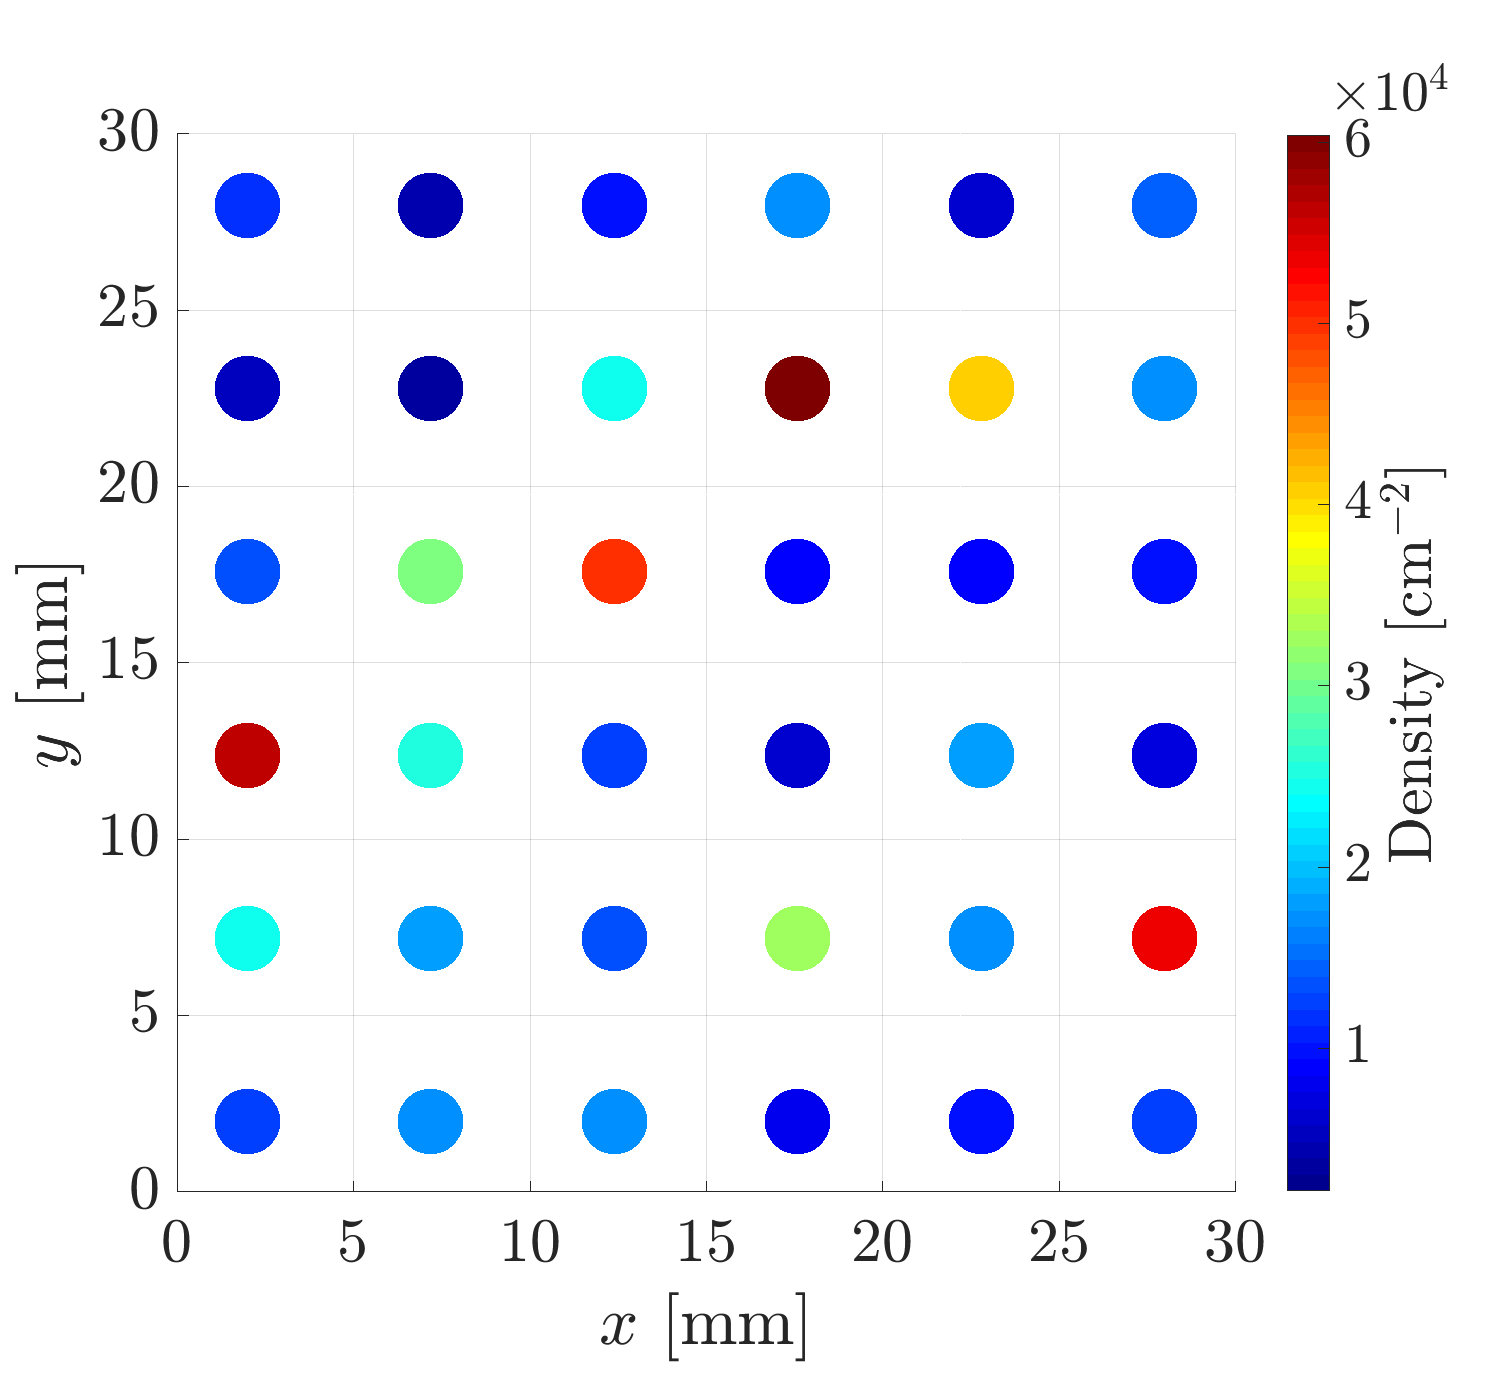
\includegraphics[width=0.5\linewidth]{LPE453_densityData.png}
    \caption[Map of the density of donut-shaped structures on the \ac{mct} film grown on substrate A.]{A map of the density of donut-shaped structures at 36 different locations on the $\SI{30}{\milli\metre}\times\SI{30}{\milli\metre}$ \ac{mct} film grown on substrate A. The density measurements were obtained by counting the number of donut-shaped defects in Nomarski optical microscopy images covering $\SI{558}{\micro\metre}\times\SI{419}{\micro\metre}$ areas. In total, \SI{0.94}{\percent} of the substrate surface was measured. The density was observed to vary between \SIrange{4e+3}{6e+4}{\centi\metre^{-2}} with an average defect density of \SI{2e+04}{\centi\metre^{-2}}.}
    \label{fig:LPE453_densityData}
\end{figure}

%The circular shape of the large defects and the donut-shaped defects indicate that they are formed while the material were liquid during \ac{lpe}

%%=========================================
%\subsection{Particles and Surface Features}
%Seven different types of particles and surface features were observed on the surface of substrate B, see Fig.~\ref{fig:subBa_sem_w_eds}. They will be described and identified in the following.

%The presence of depressions or voids, which may, or may not, retain droplets of solution, can be interpretated according to the results published by Bauser [9, E. Bauser, AppI. Phys. 15 (1978) 243]. The presence on the substrate of defects like oxide, microprecipitates, graphite particles prevents the wetting of the substrate by the liquid phase and can induce voids or depressions.Fig. 6 illustrates this mechanism.

\begin{figure}
    \centering
    \begin{subfigure}[t]{\textwidth}
        \caption{}\label{fig:subAc_donutshaped}
          \begin{minipage}[c]{0.43\linewidth}
            \centering
            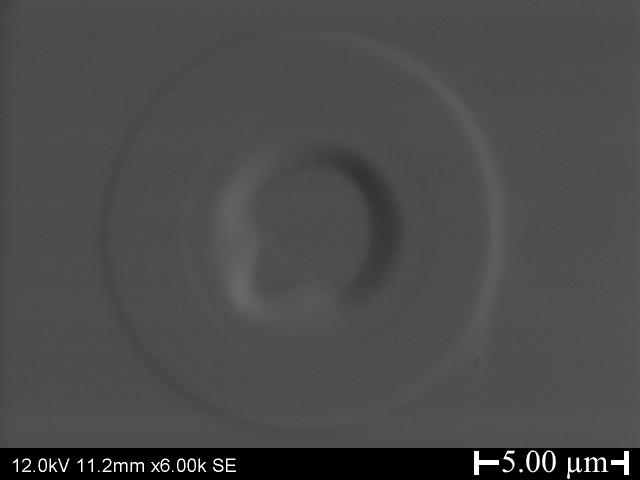
\includegraphics[width=\linewidth]{LPE453_sem_02b_m005.png}
          \end{minipage}
          \hfill
          \begin{minipage}[c]{0.43\linewidth}
            \centering
            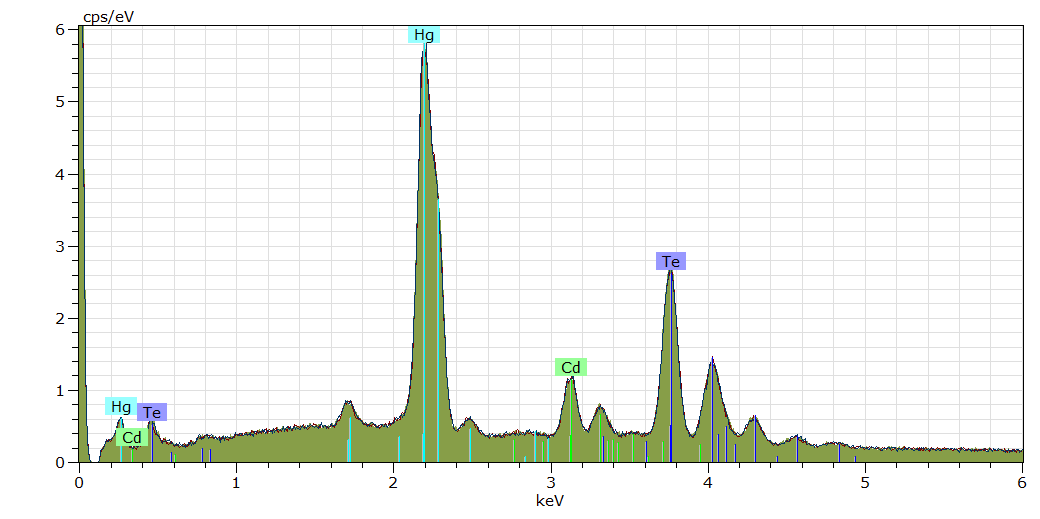
\includegraphics[width=\linewidth]{LPE453_sem_02b_m005_eds.png}
          \end{minipage}
          \begin{minipage}[c]{0.11\linewidth}
            \centering
            \atomicTable[\ce{Te} & \SI{52,05}{}][\ce{Hg}&\SI{34.78}{}][\ce{Cd}&\SI{13,18}{}]
          \end{minipage}
    \end{subfigure}
    \par\bigskip
    \begin{subfigure}[t]{\textwidth}
        \caption{}\label{fig:subAc_largecircular}
          \begin{minipage}[c]{0.43\linewidth}
            \centering
            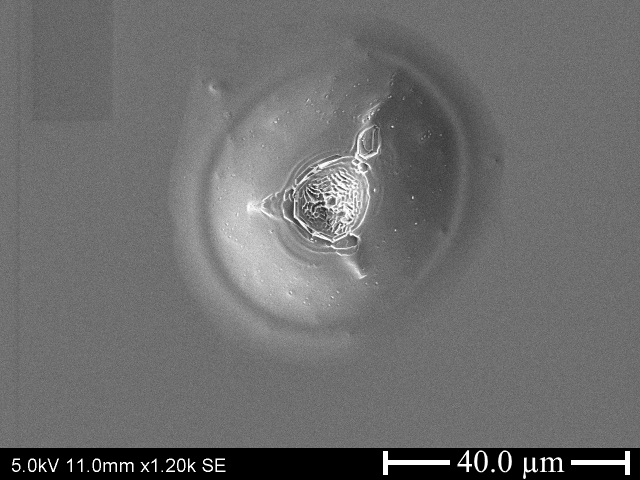
\includegraphics[width=\linewidth]{LPE453_sem_02c_m007.png}
          \end{minipage}
          \hfill
          \begin{minipage}[c]{0.43\linewidth}
            \centering
            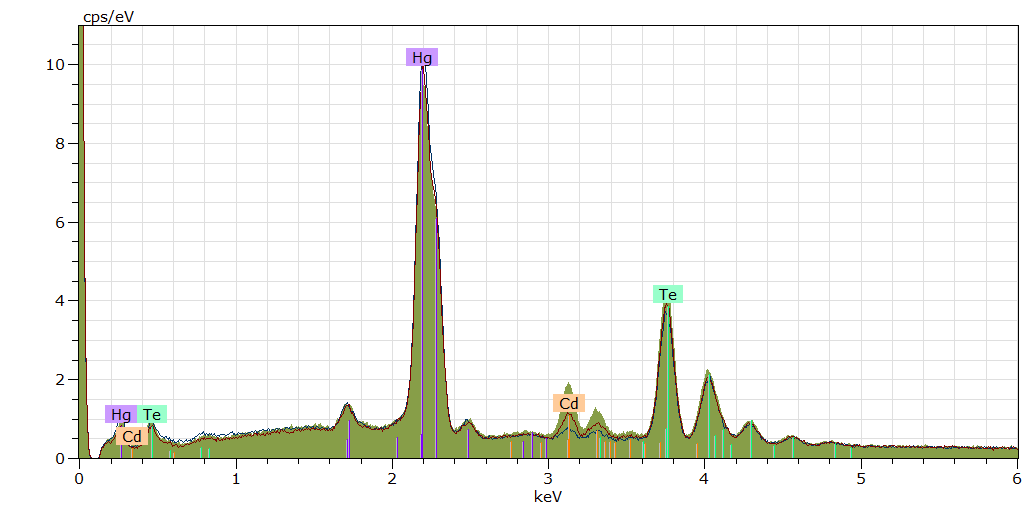
\includegraphics[width=\linewidth]{LPE453_sem_02c_m007_eds.png}
          \end{minipage}
          \begin{minipage}[c]{0.11\linewidth}
            \centering
            \atomicTable[\ce{Te} & \SI{52.23}{}][\ce{Hg}&\SI{44.21}{}][\ce{Cd}&\SI{3.55}{}]
          \end{minipage}
    \end{subfigure}
    \par\bigskip
    \begin{subfigure}[t]{\textwidth}
        \caption{}\label{fig:subAc_carbonbased}
          \begin{minipage}[c]{0.43\linewidth}
            \centering
            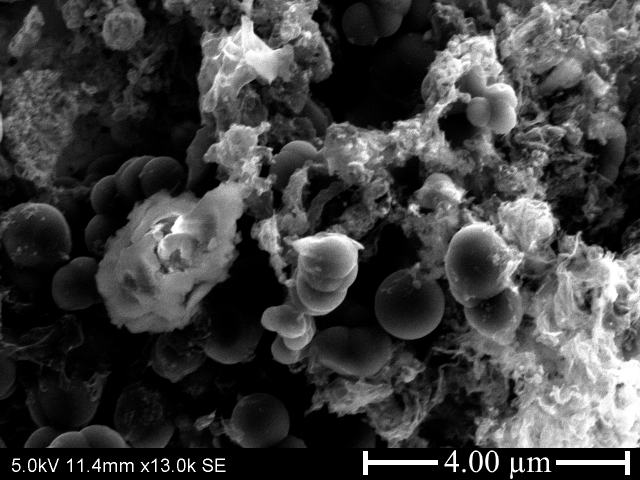
\includegraphics[width=\linewidth]{LPE453_sem_02b_m010.png}
          \end{minipage}
          \hfill
          \begin{minipage}[c]{0.43\linewidth}
            \centering
            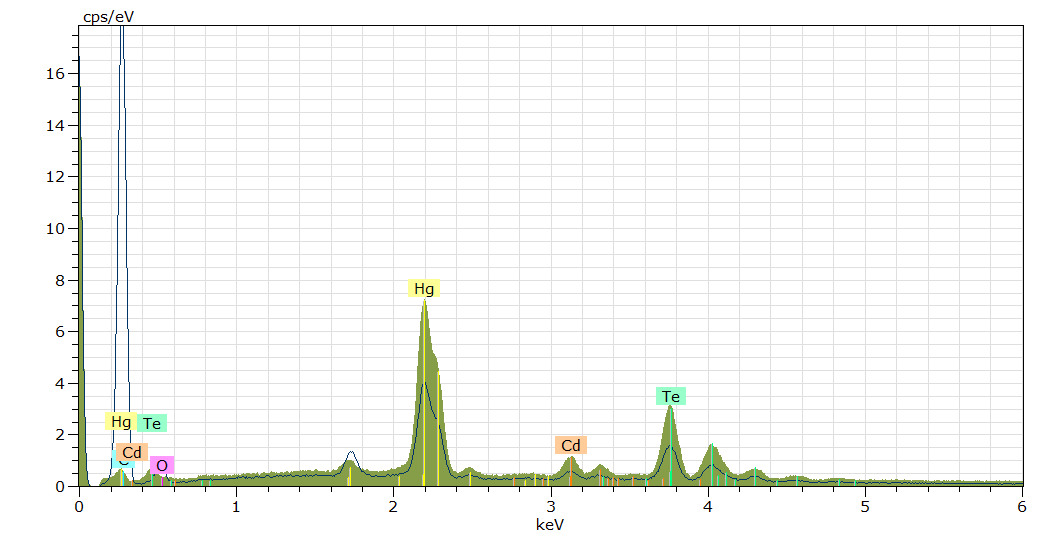
\includegraphics[width=\linewidth]{LPE453_sem_02b_m010_eds.png}
          \end{minipage}
          \begin{minipage}[c]{0.11\linewidth}
            \centering
            \atomicTable[\ce{C}&\SI{87.07}{}][\ce{Te}&\SI{4.75}{}][\ce{Hg}&\SI{3.96}{}][\ce{O}&\SI{3.58}{}][\ce{Cd}&\SI{0.64}{}]
          \end{minipage}
    \end{subfigure}
    \caption[\Ac{sem} images, \ac{eds} spectra, and \ac{eds} atomic compositions of five different types of particles and defects found on \ac{mct} film grown on substrate A.]{High-resolution \ac{sem} images of five different types of particles and defects found on the \ac{mct} film grown on substrate A and the corresponding \ac{eds} spectra and atomic compositions: \subref{fig:subAc_donutshaped} Donut-shaped defect; \subref{fig:subAc_largecircular} large cirular defect; \subref{fig:subAc_carbonbased} carbon based particles; \subref{fig:subAc_NBholder} boron nitride (\ce{B2N3}) particle; and \subref{fig:subAc_mctparticle} \ac{mct} particle. The blue line represents the \ac{eds} spectrum of the particle, while the filled green represents the \ac{eds} spectrum of the underlying substrate.}\label{fig:subAc_sem_w_eds}
\end{figure}
%
\begin{figure}[htbp]
\ContinuedFloat
    \centering
    \begin{subfigure}[t]{\textwidth}
        \caption{}\label{fig:subAc_NBholder}
          \begin{minipage}[c]{0.43\linewidth}
            \centering
            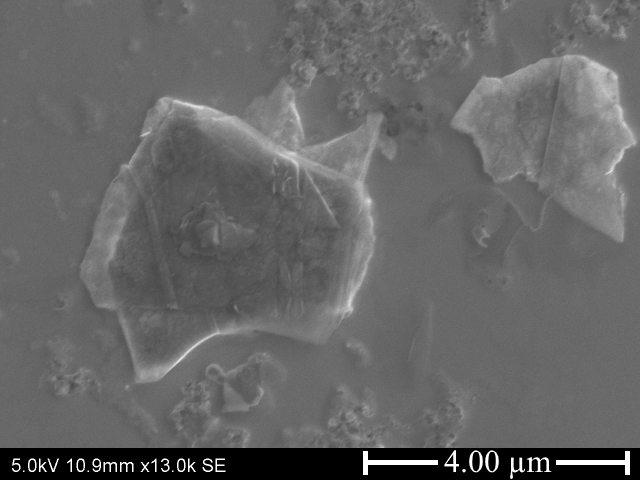
\includegraphics[width=\linewidth]{LPE453_sem_02b_m006.png}
          \end{minipage}
          \hfill
          \begin{minipage}[c]{0.43\linewidth}
            \centering
            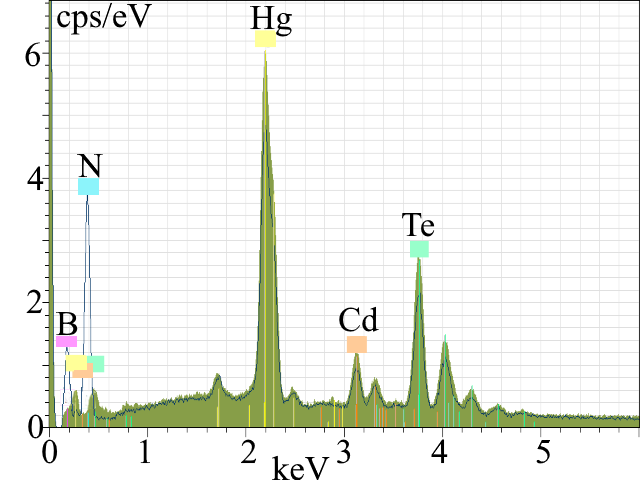
\includegraphics[width=\linewidth]{LPE453_sem_02b_m006_eds.png}
          \end{minipage}
          \begin{minipage}[c]{0.11\linewidth}
            \centering
            \atomicTable[\ce{N}&\SI{53.16}{}][\ce{B}&\SI{34.08}{}][\ce{Te}&\SI{5.98}{}][\ce{Hg}&\SI{5.33}{}][\ce{Cd}&\SI{1.45}{}]
          \end{minipage}
    \end{subfigure}
    \begin{subfigure}[t]{\textwidth}
        \caption{}\label{fig:subAc_mctparticle}
          \begin{minipage}[c]{0.43\linewidth}
            \centering
            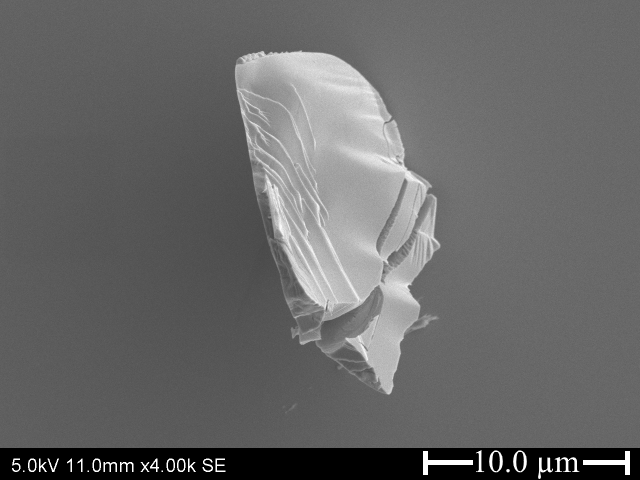
\includegraphics[width=\linewidth]{LPE453_sem_02b_m012.png}
          \end{minipage}
          \hfill
          \begin{minipage}[c]{0.43\linewidth}
            \centering
            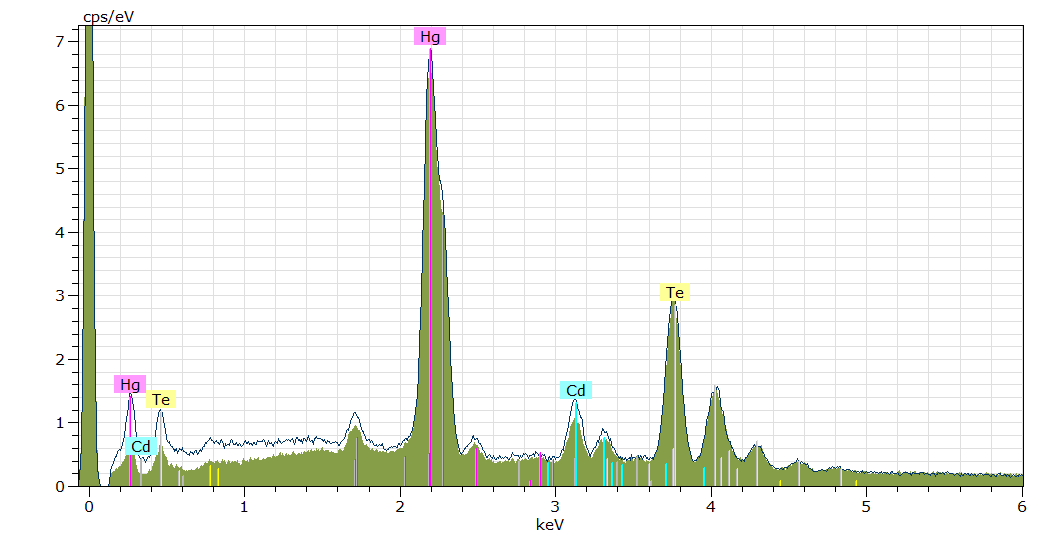
\includegraphics[width=\linewidth]{LPE453_sem_02b_m012_eds.png}
          \end{minipage}
          \begin{minipage}[c]{0.11\linewidth}
            \centering
            \atomicTable[\ce{Te} & \SI{50,47}{}][\ce{Hg}&\SI{38.51}{}][\ce{Cd}&\SI{11,01}{}]
          \end{minipage}
    \end{subfigure}
    \captionsetup{list=no}
    \caption{\emph{(continued)}}
\end{figure}

The donut-shaped defects had an elevated outer circle with a lowered centre, as seen in Fig.~\ref{fig:subAc_donutshaped}. \Ac{eds} spectra revealed that both the elevated and lowered part of the donut-shaped defect consisted of the same material as the surrounding substrate. According to \citet{radhakrishnan2003surface}, the donut-shaped defects are due to inherent substrate defects, i.e. oxides on the surface or graphite particles from the slider boat, which prevent the melt from wetting the surface, and hence, induce pits in the grown layer. %Depressions are due  to microprecipitates in the substrate.

The large circular defects were pits in the substrate surface with a bright triangular shaped inclusion/precipitate inside them, as seen in Fig.~\ref{fig:subAc_largecircular}. The \ac{eds} spectrum of the centre of the defect revealed that it consisted of \ce{HgTe}, while the \ac{eds} spectrum of the side walls of the pit revealed that they consisted of the same material as the surrounding substrate. %\todo{Skriv om: This is because, the mercury evaporation leaves a tellurium-rich phase (precipitate/inclusion) on the \ce{HgCdTe} epilayer, which is in tetrahedral shape, and when viewed from the (111)B face appears triangular \citep{pautrat1982segregation}.}

According to \citet{pelliciari1994te}, the density of large defects corresponds well with the density of tellurium precipitates in the substrate prior to growth. \citet{pelliciari1994te} measured a density of large defects twice as big as the one measured on the film grown on substrate A. \todo{Sammenlign med telling av tellurium precipitates.}

It was observed that a few of the donut-shaped defects had residual particles trapped in the middle, as seen in Fig.~\ref{fig:subAc_donut_w_particles}. The particles were found to be carbon based, see Fig.~\ref{fig:subAc_carbonbased}, and boron nitride (\ce{B2N3}), see Fig.~\ref{fig:subAc_NBholder}. Boron nitride is a part of the \ac{lpe} equipment where it keeps the substrate fixed during growth. The boron nitride piece was polished once in a while to remove residue from the growth process. It may be the debris from the polishing which had settled on the grown film.

\begin{figure}[htbp]
    \centering
    \mySubfigure{0.49\textwidth}{LPE453_sem_02b_m009.png}[fig:subAc_donut_w_particles_C]
    \hfill
    \mySubfigure{0.49\textwidth}{LPE453_sem_02c_m005.png}[fig:subAc_donut_w_particles_BN]
    \caption[\Ac{sem} images of donut-shaped defects filled with carbon based particles and boron nitride particles.]{\Ac{sem} images of donut-shaped defects filled with \subref{fig:subAc_donut_w_particles_C} carbon based particles and \subref{fig:subAc_donut_w_particles_BN} boron nitride particles seen on \ac{mct} film grown by \ac{lpe} on (111)B-oriented substrate A.}
    \label{fig:subAc_donut_w_particles}
\end{figure}

In addition to the particles found in connection with the donut-shaped defects, some \ac{mct} particles were found near the upper left corner of the substrate, see Fig.~\ref{fig:subAc_mctparticle}.

%%=========================================
\subsection{Composition and Thickness}

\todo{FTIR: correlate with polishing grit or donut density.}

\begin{figure}[htbp]
    \centering
    \mySubfigure{0.60175438596\linewidth}{LPE453_ftir_spectra.png}[fig:subAc_ftir_spectra]
    \hfill
    \mySubfigure{0.37824561403\linewidth}{LPE453_ftir_transmission_at_k500cm-1.png}[fig:subAc_ftir_map_500cm-1]
    \caption[\Ac{ftir} measurements of the \ac{mct} film grown on substrate A.]{\Ac{ftir} measurements recorded from a $11\times11$ grid on the $\SI{30}{\milli\metre}\times\SI{30}{\milli\metre}$ \ac{mct} film grown on substrate A: \subref{fig:subAc_ftir_spectra} Transmission spectra; \subref{fig:subAc_ftir_map_500cm-1} transmission map at wavenumber $k=\SI{500}{\centi\metre^{-1}}$ showing the transmittance $T$ in percentage of incoming light at each grid point.}
\end{figure}

%%=========================================
\subsection{Impurity Analysis -- EDS}

\Ac{eds} was used to get a quantitative analysis of the chemical composition of the \ac{mct} film grown by \ac{lpe} on substrate A. The results can be seen in Table~\ref{tab:subAc_eds_analysis}. The following elements were identified: \ce{Te}, \ce{Hg}, \ce{Cd}, \ce{C}, \ce{O}, and \ce{Al}. The relative concentrations of \ce{Cd}, \ce{Zn}, and \ce{Te} were \ce{Hg_{0.71}Cd_{0.29}Te}, \ce{Hg_{0.77}Cd_{0.23}Te}, and \ce{Hg_{0.76}Cd_{0.24}Te} for the centre, edge, and corner respectively. 

\begin{table}[htbp]
    \centering
    \caption[\Ac{eds} impurity analysis of \ac{mct} film grown by \ac{lpe} on substrate A.]{Results of the \ac{eds} impurity analysis at three different locations on the $\SI{30}{\milli\metre}\times\SI{30}{\milli\metre}$ \ac{mct} film grown by \ac{lpe} on (111)B-oriented substrate A (atomic concentration \%). The X-ray signal was acquired from $\SI{1270}{\micro\metre}\times\SI{890}{\micro\metre}$ areas near the centre, upper edge, and upper left corner.}\label{tab:subAc_eds_analysis}
   \begin{tabu} to 1.0\textwidth { X[1.85, r] X[1.125,c] X[1.125,c] X[1.125,c] X[1.125,c] X[1.125,c] X[1.125,c] }
        \hline
            & \textbf{\ce{Te}} (at.\%) & \textbf{\ce{Hg}} (at.\%) & \textbf{\ce{Cd}} (at.\%) & \textbf{\ce{C} } (at.\%) & \textbf{\,\ce{O}\,} (at.\%) & \textbf{\ce{Al}} (at.\%) \\
        \hline
        Near centre & \SI{43,96}{} & \SI{30,82}{} & \SI{12,39}{} & \SI{11,38}{} & \SI{1,28}{} & \SI{0,17}{} \\
        Near edge & \SI{43,87}{} & \SI{33,27}{} & \SI{9,80}{} & \SI{11,70}{} & \SI{1,13}{} & \SI{0,23}{} \\
        Near corner & \SI{43,58}{} & \SI{32,74}{} & \SI{10,24}{} & \SI{11,98	}{} & \SI{1,18}{} & \SI{0,27}{}  \\
        \hline
    \end{tabu}
\end{table}
%%=========================================